The history of software security is characterized by a continuous cycle of new attack avenues and corresponding defensive responses.
This co-evolutionary process has led to a landscape of highly sophisticated memory corruption exploits and mitigations.
A particularly common and dangerous class of memory corruption exploits is \glspl{CRA} and their---now mostly obsolete---predecessor code-injection attacks.

Code-injection attacks and \glspl{CRA} typically proceed in three phases:
\begin{inline}
    \item a reconnaissance phase where the attacker collects information about the target, such as addresses of target code,
    \item a memory corruption to overwrite control-flow data and
    \item the malicious code execution that transfers control to attacker-chosen code.
\end{inline}
Defenses against such attacks fall into three categories:
\begin{itemize}
    \item memory-safety enforcement;
    \item control-flow enforcement;
    \item randomization.
\end{itemize}
Each defense category targets a different step of the attack.
Memory-safety enforcement aims to prevent the memory corruption required to divert the control flow.
Control-flow enforcement tolerates the memory corruption but tries to lock the attacker into a previously determined control-flow graph.
Randomization-based techniques, also called software diversity, aim to disrupt the attacker's reconnaissance phase by invalidating a priori knowledge the attacker has about the target.

Increasingly sophisticated \gls{CRA} variants have driven the evolution of defenses in each category.
The following sections trace the historical development of \glspl{CRA} together with the development of defenses in each category.
\cref{fig:coevolution-epoch-all} shows the complete timeline for important \glspl{CRA} and defenses and each of the following sections looks at an epoch in this timeline in more detail.



\begin{figure}[p]
    \centering
    \resizebox{!}{0.95\textheight}{%
        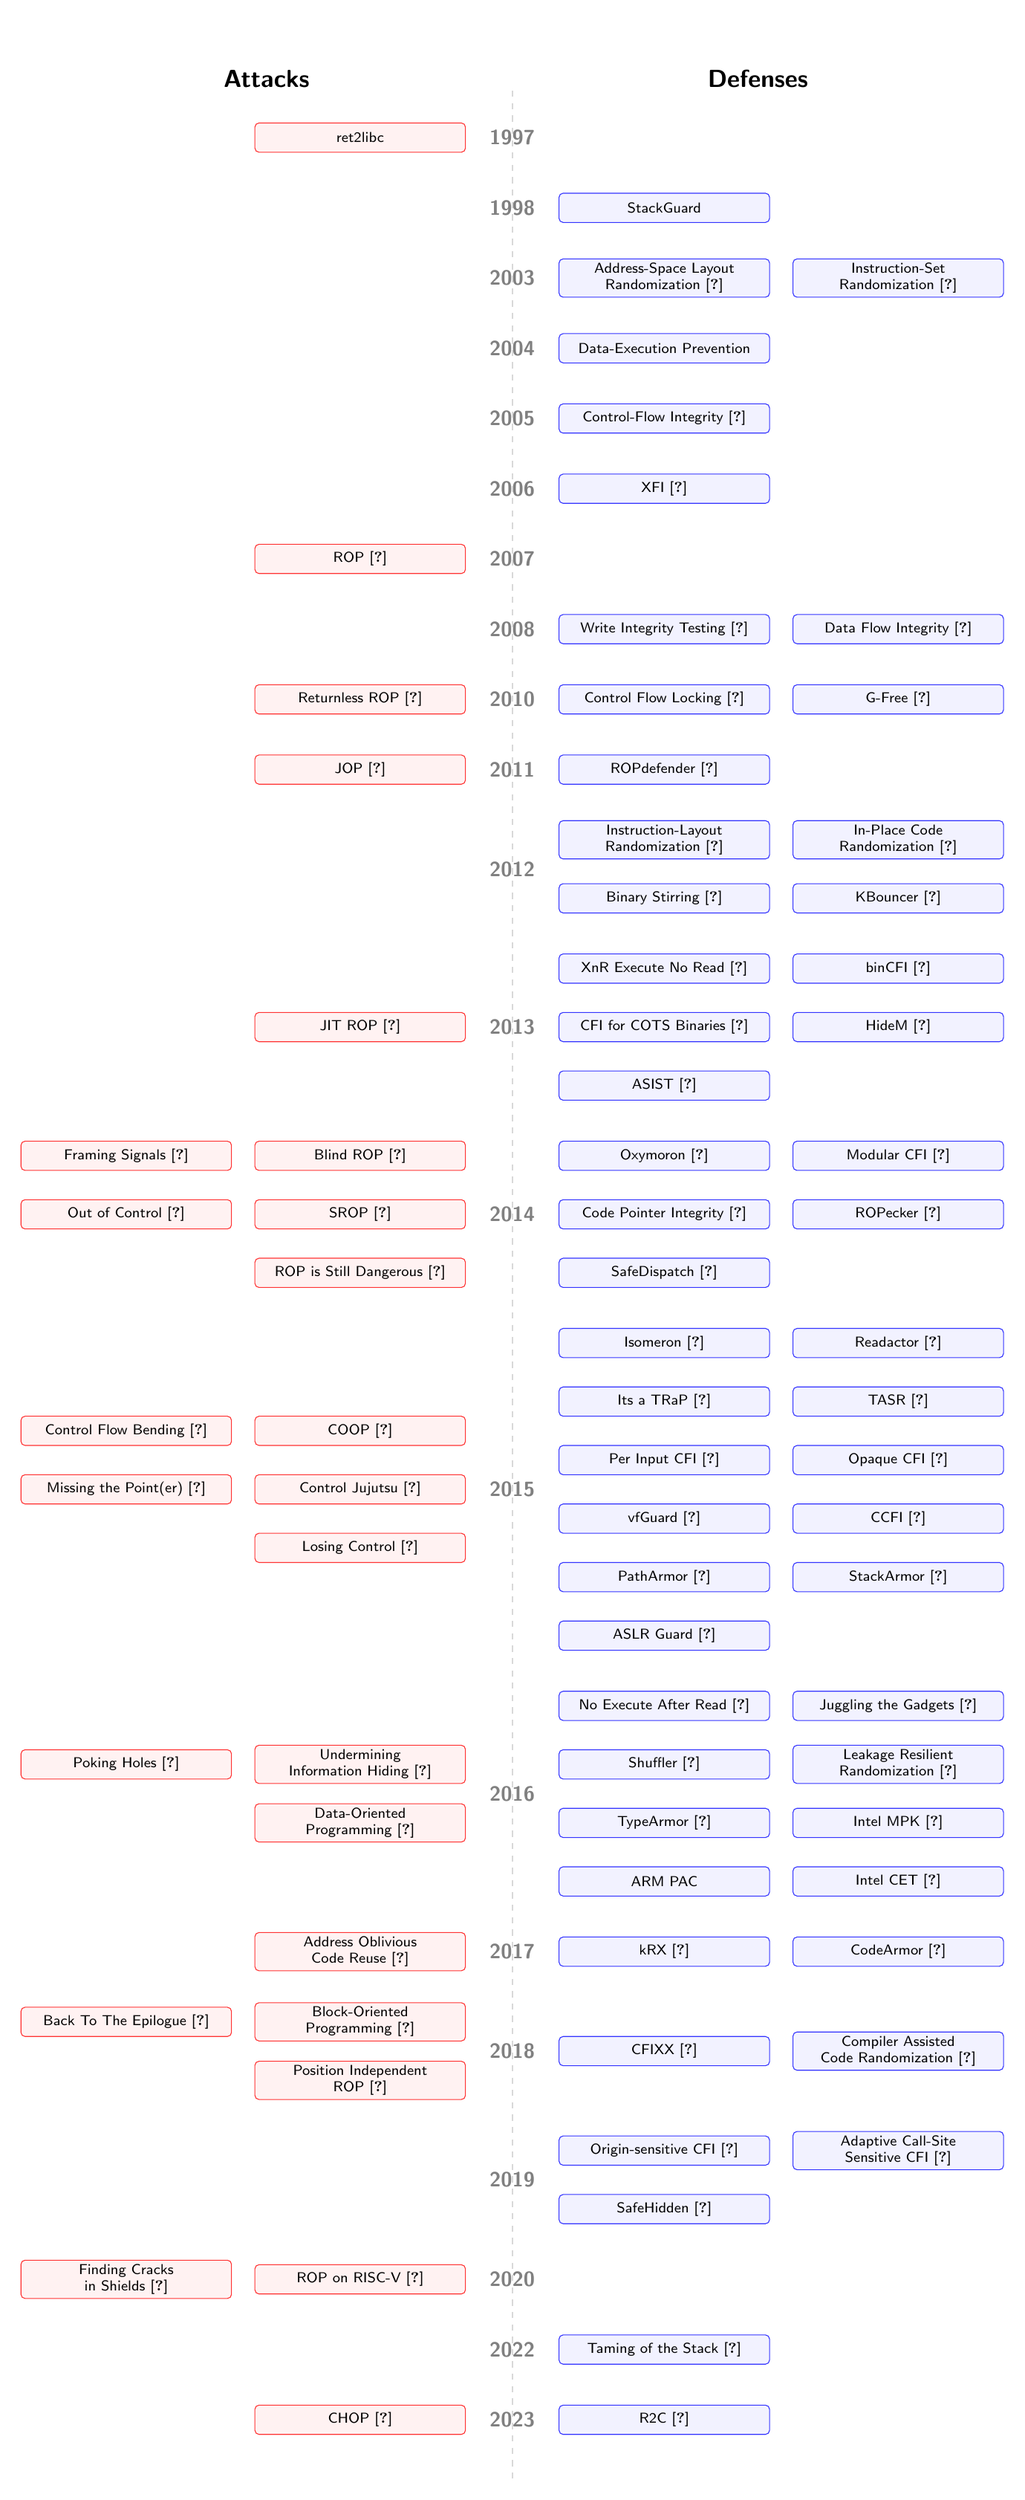
\begin{tikzpicture}[year node/.style={font=\bfseries\sffamily\color{gray}, align=center, inner sep=2pt},attack node/.style={draw=red!80, fill=red!5, rounded corners=2pt, font=\scriptsize\sffamily, align=center, minimum width=3.60cm, minimum height=0.5cm, inner sep=2pt, text width=3.40cm, execute at begin node=\setlength{\emergencystretch}{0pt}\tolerance 200\hyphenpenalty 10000\exhyphenpenalty 10000},defense node/.style={draw=blue!80, fill=blue!5, rounded corners=2pt, font=\scriptsize\sffamily, align=center, minimum width=3.60cm, minimum height=0.5cm, inner sep=2pt, text width=3.40cm, execute at begin node=\setlength{\emergencystretch}{0pt}\tolerance 200\hyphenpenalty 10000\exhyphenpenalty 10000},spine/.style={thick, gray!30, dashed}]%
\node[font=\large\bfseries\sffamily] at (-4.2,1.0) {Attacks};%
\node[font=\large\bfseries\sffamily] at (4.2,1.0) {Defenses};%
  % Year 1997%
\node[year node] at (0.0,0.0) {1997};%
\node[attack node] at (-2.6,0.0) {ret2libc};%
  % Year 1998%
\node[year node] at (0.0,-1.2) {1998};%
\node[defense node] at (2.6,-1.2) {StackGuard};%
  % Year 2003%
\node[year node] at (0.0,-2.4) {2003};%
\node[defense node] at (2.6,-2.4) {Address{-}Space Layout\\ Randomization \allowbreak\cite{PaXTeam2003}};%
\node[defense node] at (6.6,-2.4) {Instruction{-}Set\\ Randomization \allowbreak\cite{boyd2010}};%
  % Year 2004%
\node[year node] at (0.0,-3.6) {2004};%
\node[defense node] at (2.6,-3.6) {Data{-}Execution Prevention};%
  % Year 2005%
\node[year node] at (0.0,-4.8) {2005};%
\node[defense node] at (2.6,-4.8) {Control{-}Flow Integrity \allowbreak\cite{Abadi2005}};%
  % Year 2006%
\node[year node] at (0.0,-6.0) {2006};%
\node[defense node] at (2.6,-6.0) {XFI \allowbreak\cite{Erlingsson2006}};%
  % Year 2007%
\node[year node] at (0.0,-7.2) {2007};%
\node[attack node] at (-2.6,-7.2) {ROP \allowbreak\cite{Shacham2007}};%
  % Year 2008%
\node[year node] at (0.0,-8.4) {2008};%
\node[defense node] at (2.6,-8.4) {Write Integrity Testing \allowbreak\cite{Akritidis2008}};%
\node[defense node] at (6.6,-8.4) {Data Flow Integrity \allowbreak\cite{castro2006}};%
  % Year 2010%
\node[year node] at (0.0,-9.6) {2010};%
\node[attack node] at (-2.6,-9.6) {Returnless ROP \allowbreak\cite{checkoway2010}};%
\node[defense node] at (2.6,-9.6) {Control Flow Locking \allowbreak\cite{Bletsch2011b}};%
\node[defense node] at (6.6,-9.6) {G{-}Free \allowbreak\cite{Onarlioglu2010}};%
  % Year 2011%
\node[year node] at (0.0,-10.8) {2011};%
\node[attack node] at (-2.6,-10.8) {JOP \allowbreak\cite{Bletsch2011a}};%
\node[defense node] at (2.6,-10.8) {ROPdefender \allowbreak\cite{davi2011}};%
  % Year 2012%
\node[year node] at (0.0,-12.5) {2012};%
\node[defense node] at (2.6,-12.0) {Instruction{-}Layout\\ Randomization \allowbreak\cite{Hiser2012}};%
\node[defense node] at (6.6,-12.0) {In{-}Place Code\\ Randomization \allowbreak\cite{Pappas2012a}};%
\node[defense node] at (2.6,-13.0) {Binary Stirring \allowbreak\cite{Wartell2012}};%
\node[defense node] at (6.6,-13.0) {KBouncer \allowbreak\cite{Pappas2013b}};%
  % Year 2013%
\node[year node] at (0.0,-15.2) {2013};%
\node[attack node] at (-2.6,-15.2) {JIT ROP \allowbreak\cite{Snow2013}};%
\node[defense node] at (2.6,-14.2) {XnR Execute No Read \allowbreak\cite{Backes2013}};%
\node[defense node] at (6.6,-14.2) {binCFI \allowbreak\cite{zhang2013}};%
\node[defense node] at (2.6,-15.2) {CFI for COTS Binaries \allowbreak\cite{zhang2013}};%
\node[defense node] at (6.6,-15.2) {HideM \allowbreak\cite{Goktas2016b}};%
\node[defense node] at (2.6,-16.2) {ASIST \allowbreak\cite{papadogiannakis2013}};%
  % Year 2014%
\node[year node] at (0.0,-18.4) {2014};%
\node[attack node] at (-2.6,-17.4) {Blind ROP \allowbreak\cite{Bittau2014a}};%
\node[attack node] at (-6.6,-17.4) {Framing Signals \allowbreak\cite{Bittau2014a}};%
\node[attack node] at (-2.6,-18.4) {SROP \allowbreak\cite{bosman2014}};%
\node[attack node] at (-6.6,-18.4) {Out of Control \allowbreak\cite{Goktas2016b}};%
\node[attack node] at (-2.6,-19.4) {ROP is Still Dangerous \allowbreak\cite{carlini2014}};%
\node[defense node] at (2.6,-17.4) {Oxymoron \allowbreak\cite{Backes2014f}};%
\node[defense node] at (6.6,-17.4) {Modular CFI \allowbreak\cite{niu2014}};%
\node[defense node] at (2.6,-18.4) {Code Pointer Integrity \allowbreak\cite{Kuznetsov2014}};%
\node[defense node] at (6.6,-18.4) {ROPecker \allowbreak\cite{Cheng2014}};%
\node[defense node] at (2.6,-19.4) {SafeDispatch \allowbreak\cite{jang2014}};%
  % Year 2015%
\node[year node] at (0.0,-23.1) {2015};%
\node[attack node] at (-2.6,-22.1) {COOP \allowbreak\cite{Schuster2015a}};%
\node[attack node] at (-6.6,-22.1) {Control Flow Bending \allowbreak\cite{Carlini2015}};%
\node[attack node] at (-2.6,-23.1) {Control Jujutsu \allowbreak\cite{Evans2015a}};%
\node[attack node] at (-6.6,-23.1) {Missing the Point(er) \allowbreak\cite{Evans2015}};%
\node[attack node] at (-2.6,-24.1) {Losing Control \allowbreak\cite{conti2015}};%
\node[defense node] at (2.6,-20.6) {Isomeron \allowbreak\cite{Davi2015}};%
\node[defense node] at (6.6,-20.6) {Readactor \allowbreak\cite{Crane2015}};%
\node[defense node] at (2.6,-21.6) {Its a TRaP \allowbreak\cite{Crane2015b}};%
\node[defense node] at (6.6,-21.6) {TASR \allowbreak\cite{bigelow2015}};%
\node[defense node] at (2.6,-22.6) {Per Input CFI \allowbreak\cite{Niu2015}};%
\node[defense node] at (6.6,-22.6) {Opaque CFI \allowbreak\cite{Mohan2015}};%
\node[defense node] at (2.6,-23.6) {vfGuard \allowbreak\cite{Prakash2015}};%
\node[defense node] at (6.6,-23.6) {CCFI \allowbreak\cite{Mashtizadeh2015}};%
\node[defense node] at (2.6,-24.6) {PathArmor \allowbreak\cite{Goktas2016b}};%
\node[defense node] at (6.6,-24.6) {StackArmor \allowbreak\cite{Chen2015c}};%
\node[defense node] at (2.6,-25.6) {ASLR Guard \allowbreak\cite{Lu2015}};%
  % Year 2016%
\node[year node] at (0.0,-28.3) {2016};%
\node[attack node] at (-2.6,-27.8) {Undermining\\ Information Hiding \allowbreak\cite{Goktas2016}};%
\node[attack node] at (-6.6,-27.8) {Poking Holes \allowbreak\cite{Oikonomopoulos2016a}};%
\node[attack node] at (-2.6,-28.8) {Data{-}Oriented\\ Programming \allowbreak\cite{Hu2016}};%
\node[defense node] at (2.6,-26.8) {No Execute After Read \allowbreak\cite{Werner2016}};%
\node[defense node] at (6.6,-26.8) {Juggling the Gadgets \allowbreak\cite{koo2016}};%
\node[defense node] at (2.6,-27.8) {Shuffler \allowbreak\cite{WilliamsKing2016}};%
\node[defense node] at (6.6,-27.8) {Leakage Resilient\\ Randomization \allowbreak\cite{Braden2016}};%
\node[defense node] at (2.6,-28.8) {TypeArmor \allowbreak\cite{VanderVeen2015b}};%
\node[defense node] at (6.6,-28.8) {Intel MPK \allowbreak\cite{Wahbe1993}};%
\node[defense node] at (2.6,-29.8) {ARM PAC};%
\node[defense node] at (6.6,-29.8) {Intel CET \allowbreak\cite{IntelCET}};%
  % Year 2017%
\node[year node] at (0.0,-31.0) {2017};%
\node[attack node] at (-2.6,-31.0) {Address Oblivious\\ Code Reuse \allowbreak\cite{Rudd2017}};%
\node[defense node] at (2.6,-31.0) {kRX \allowbreak\cite{Pomonis2019}};%
\node[defense node] at (6.6,-31.0) {CodeArmor \allowbreak\cite{Chen2017a}};%
  % Year 2018%
\node[year node] at (0.0,-32.7) {2018};%
\node[attack node] at (-2.6,-32.2) {Block{-}Oriented\\ Programming \allowbreak\cite{Ispoglou2018}};%
\node[attack node] at (-6.6,-32.2) {Back To The Epilogue \allowbreak\cite{biondo2018}};%
\node[attack node] at (-2.6,-33.2) {Position Independent\\ ROP \allowbreak\cite{Goktas2018}};%
\node[defense node] at (2.6,-32.7) {CFIXX \allowbreak\cite{Burow2018CFIXX}};%
\node[defense node] at (6.6,-32.7) {Compiler Assisted\\ Code Randomization \allowbreak\cite{Koo2018}};%
  % Year 2019%
\node[year node] at (0.0,-34.9) {2019};%
\node[defense node] at (2.6,-34.4) {Origin{-}sensitive CFI \allowbreak\cite{khandaker2019}};%
\node[defense node] at (6.6,-34.4) {Adaptive Call{-}Site\\ Sensitive CFI \allowbreak\cite{khandaker2019a}};%
\node[defense node] at (2.6,-35.4) {SafeHidden \allowbreak\cite{wang2019a}};%
  % Year 2020%
\node[year node] at (0.0,-36.6) {2020};%
\node[attack node] at (-2.6,-36.6) {ROP on RISC{-}V \allowbreak\cite{jaloyan2020}};%
\node[attack node] at (-6.6,-36.6) {Finding Cracks\\ in Shields \allowbreak\cite{li2020}};%
  % Year 2022%
\node[year node] at (0.0,-37.8) {2022};%
\node[defense node] at (2.6,-37.8) {Taming of the Stack \allowbreak\cite{huang2022a}};%
  % Year 2023%
\node[year node] at (0.0,-39.0) {2023};%
\node[attack node] at (-2.6,-39.0) {CHOP \allowbreak\cite{duta2023}};%
\node[defense node] at (2.6,-39.0) {R2C \allowbreak\cite{berlakovich2023}};%
\path[spine,draw] (0.0,0.8) -- (0.0,-40.0);%
\path[use as bounding box] (-8.40,-40.00) rectangle (8.40,2.00);%
\end{tikzpicture}%
    }
    \caption{Timeline for code-injection attacks and defenses (1997--Present).}
    \label{fig:coevolution-epoch-all}
\end{figure}


\FloatBarrier
\begin{figure}[H]
    \centering
    \resizebox{\textwidth}{!}{%
        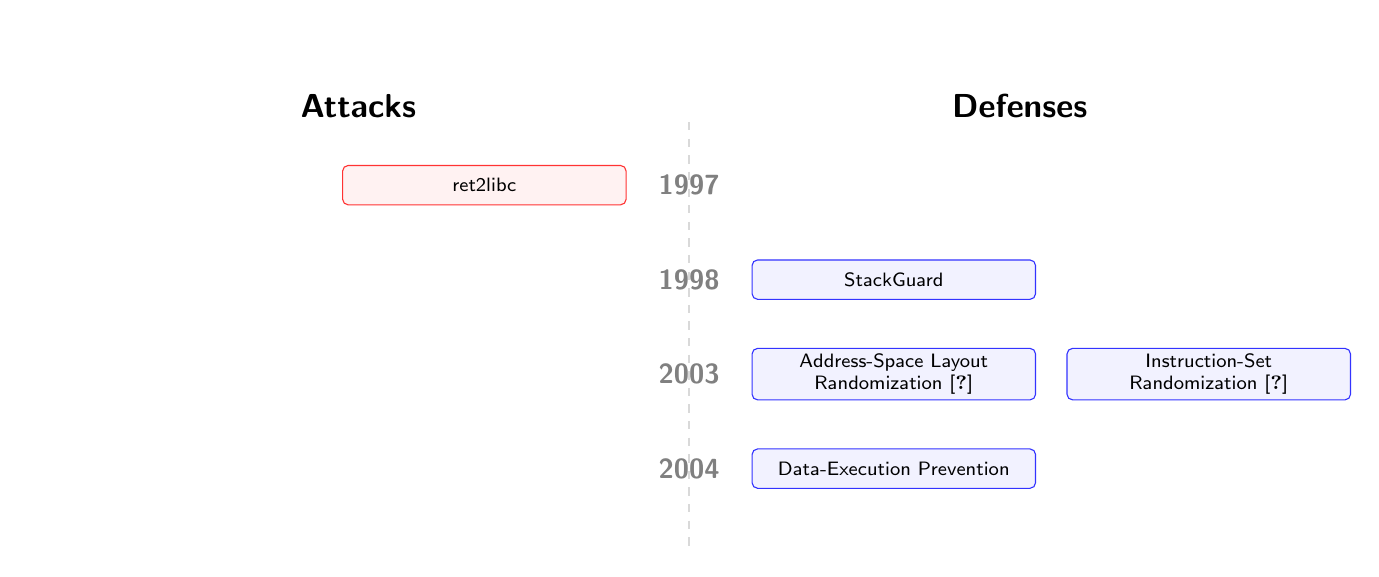
\begin{tikzpicture}[year node/.style={font=\bfseries\sffamily\color{gray}, align=center, inner sep=2pt},attack node/.style={draw=red!80, fill=red!5, rounded corners=2pt, font=\scriptsize\sffamily, align=center, minimum width=3.60cm, minimum height=0.5cm, inner sep=2pt, text width=3.40cm, execute at begin node=\setlength{\emergencystretch}{0pt}\tolerance 200\hyphenpenalty 10000\exhyphenpenalty 10000},defense node/.style={draw=blue!80, fill=blue!5, rounded corners=2pt, font=\scriptsize\sffamily, align=center, minimum width=3.60cm, minimum height=0.5cm, inner sep=2pt, text width=3.40cm, execute at begin node=\setlength{\emergencystretch}{0pt}\tolerance 200\hyphenpenalty 10000\exhyphenpenalty 10000},spine/.style={thick, gray!30, dashed}]%
\node[font=\large\bfseries\sffamily] at (-4.2,1.0) {Attacks};%
\node[font=\large\bfseries\sffamily] at (4.2,1.0) {Defenses};%
  % Year 1997%
\node[year node] at (0.0,0.0) {1997};%
\node[attack node] at (-2.6,0.0) {ret2libc};%
  % Year 1998%
\node[year node] at (0.0,-1.2) {1998};%
\node[defense node] at (2.6,-1.2) {StackGuard};%
  % Year 2003%
\node[year node] at (0.0,-2.4) {2003};%
\node[defense node] at (2.6,-2.4) {Address{-}Space Layout\\ Randomization \allowbreak\cite{PaXTeam2003}};%
\node[defense node] at (6.6,-2.4) {Instruction{-}Set\\ Randomization \allowbreak\cite{boyd2010}};%
  % Year 2004%
\node[year node] at (0.0,-3.6) {2004};%
\node[defense node] at (2.6,-3.6) {Data{-}Execution Prevention};%
\path[spine,draw] (0.0,0.8) -- (0.0,-4.6);%
\path[use as bounding box] (-8.40,-4.60) rectangle (8.40,2.00);%
\end{tikzpicture}%
    }
    \caption{Epoch timeline for code-injection attacks and defenses (1997--2004).}
    \label{fig:coevolution-epoch-code-injection}
\end{figure}
\section{Code Injection (1997--2004)}
\label{sec:epoch-injection}
In the earliest era (1997--2004), the adversary's primary goal was to inject new code (\eg shellcode) into the target process' memory space and subsequently redirect execution to the injected code.
Despite the possibility of code injection in the early days, a form of \gls{CRA} called \propername{return-to-libc} was described already in 1997.
\propername{Return-to-libc} operates on the function level and reuses functions from the standard C library.
These functions are both powerful and likely present in most attacked programs.

To counter these early attacks, several randomization-based techniques were proposed.
\propername{StackGuard} protects return addresses against buffer overflows with \enquote{canaries}---random values checked before a function returns.
Based on the observation that an attacker needs exact addresses both for injection and reuse, \gls{ASLR} was introduced to randomize the base addresses of the stack, heap and libraries~\cite{PaXTeam2003}.
Full adoption of \gls{ASLR} took years, however, as it requires position-independent code.
Another issue with \gls{ASLR} is that a 32-bit address space does not offer enough entropy, and even in a 64-bit address space, pointer leaks and side-channels make \gls{ASLR} vulnerable~\cite{Gras2017}.
Even ten years later, \gls{ASLR} implementations still suffer from severe limitations~\cite{binosi2024}.
Research into \gls{ISR} explored randomizing the processor's instruction set to prevent the execution of injected code~\cite{boyd2010,papadogiannakis2013}.

At around 2004, the introduction of a new \gls{CPU} feature made it practical to prevent memory regions from being writable and executable at the same time.
The memory-safety enforcement mechanism leveraging this \gls{CPU} feature is known as \wox or \gls{DEP}.
With the widespread adoption of \gls{DEP}, attackers were forced to switch to more advanced forms of \glspl{CRA}.

\FloatBarrier
\begin{figure}[H]
    \centering
    \resizebox{\textwidth}{!}{%
        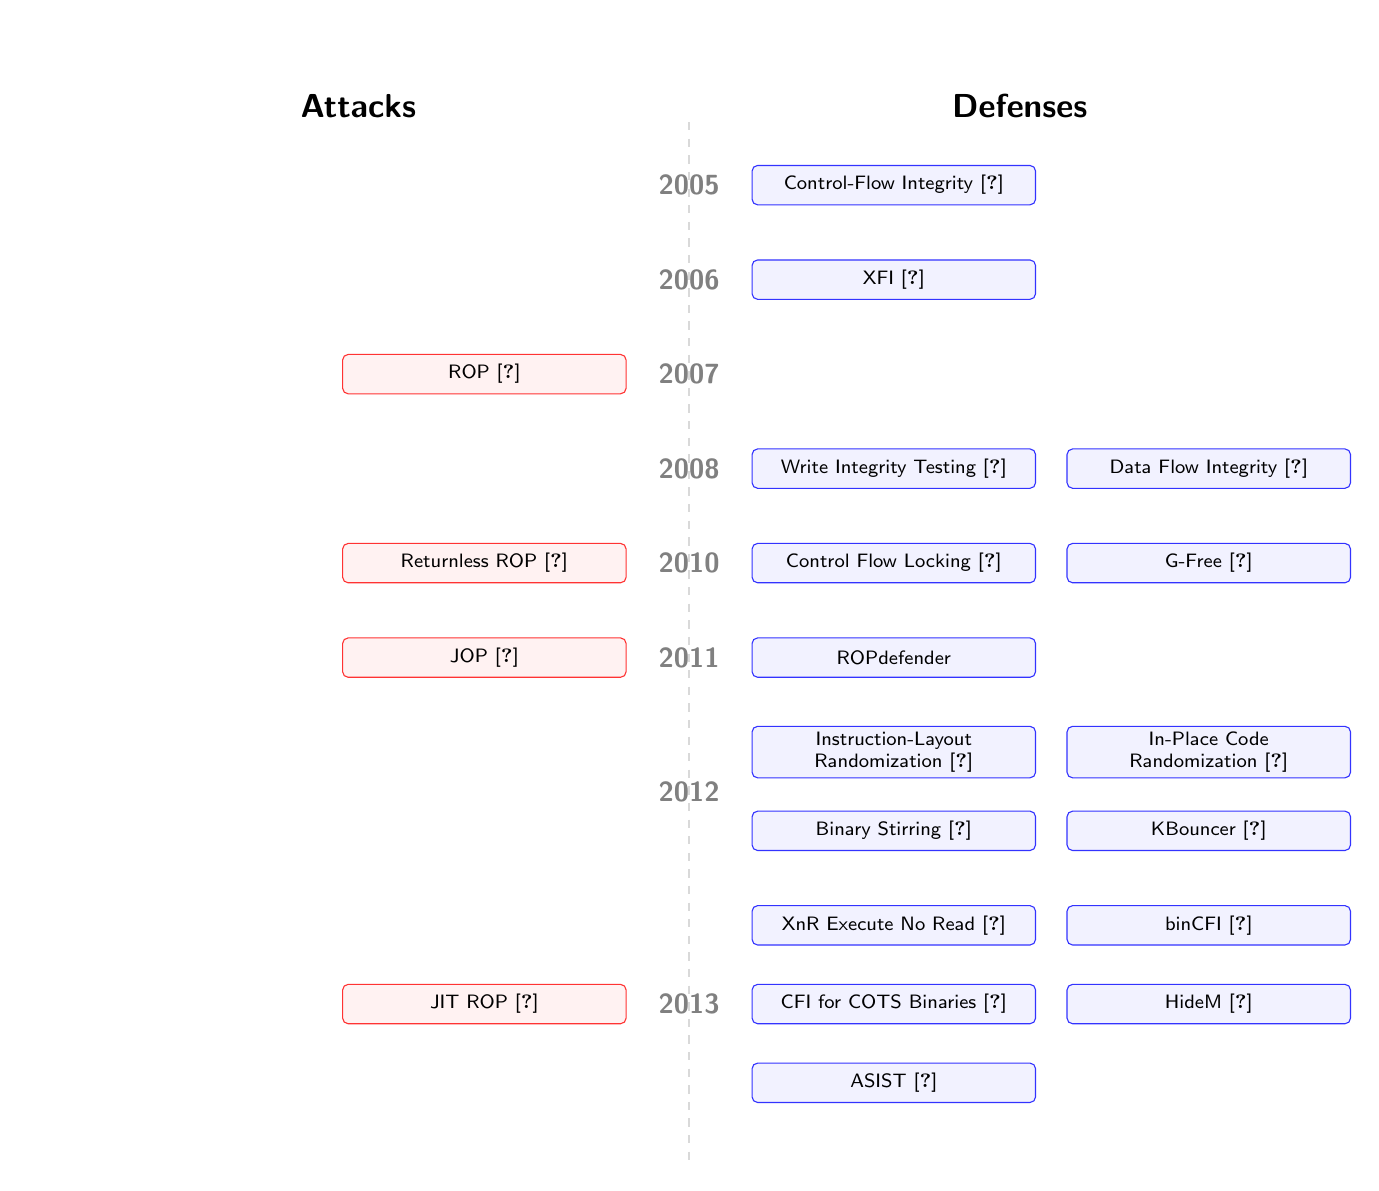
\begin{tikzpicture}[year node/.style={font=\bfseries\sffamily\color{gray}, align=center, inner sep=2pt},attack node/.style={draw=red!80, fill=red!5, rounded corners=2pt, font=\scriptsize\sffamily, align=center, minimum width=3.60cm, minimum height=0.5cm, inner sep=2pt, text width=3.40cm, execute at begin node=\setlength{\emergencystretch}{0pt}\tolerance 200\hyphenpenalty 10000\exhyphenpenalty 10000},defense node/.style={draw=blue!80, fill=blue!5, rounded corners=2pt, font=\scriptsize\sffamily, align=center, minimum width=3.60cm, minimum height=0.5cm, inner sep=2pt, text width=3.40cm, execute at begin node=\setlength{\emergencystretch}{0pt}\tolerance 200\hyphenpenalty 10000\exhyphenpenalty 10000},spine/.style={thick, gray!30, dashed}]%
\node[font=\large\bfseries\sffamily] at (-4.2,1.0) {Attacks};%
\node[font=\large\bfseries\sffamily] at (4.2,1.0) {Defenses};%
  % Year 2005%
\node[year node] at (0.0,0.0) {2005};%
\node[defense node] at (2.6,0.0) {Control{-}Flow Integrity \allowbreak\cite{Abadi2005}};%
  % Year 2006%
\node[year node] at (0.0,-1.2) {2006};%
\node[defense node] at (2.6,-1.2) {XFI \allowbreak\cite{Erlingsson2006}};%
  % Year 2007%
\node[year node] at (0.0,-2.4) {2007};%
\node[attack node] at (-2.6,-2.4) {ROP \allowbreak\cite{Shacham2007}};%
  % Year 2008%
\node[year node] at (0.0,-3.6) {2008};%
\node[defense node] at (2.6,-3.6) {Write Integrity Testing \allowbreak\cite{Akritidis2008}};%
\node[defense node] at (6.6,-3.6) {Data Flow Integrity \allowbreak\cite{castro2006}};%
  % Year 2010%
\node[year node] at (0.0,-4.8) {2010};%
\node[attack node] at (-2.6,-4.8) {Returnless ROP \allowbreak\cite{checkoway2010}};%
\node[defense node] at (2.6,-4.8) {Control Flow Locking \allowbreak\cite{Bletsch2011b}};%
\node[defense node] at (6.6,-4.8) {G{-}Free \allowbreak\cite{Onarlioglu2010}};%
  % Year 2011%
\node[year node] at (0.0,-6.0) {2011};%
\node[attack node] at (-2.6,-6.0) {JOP \allowbreak\cite{Bletsch2011a}};%
\node[defense node] at (2.6,-6.0) {ROPdefender};%
  % Year 2012%
\node[year node] at (0.0,-7.7) {2012};%
\node[defense node] at (2.6,-7.2) {Instruction{-}Layout\\ Randomization \allowbreak\cite{Hiser2012}};%
\node[defense node] at (6.6,-7.2) {In{-}Place Code\\ Randomization \allowbreak\cite{Pappas2012a}};%
\node[defense node] at (2.6,-8.2) {Binary Stirring \allowbreak\cite{Wartell2012}};%
\node[defense node] at (6.6,-8.2) {KBouncer \allowbreak\cite{Pappas2013b}};%
  % Year 2013%
\node[year node] at (0.0,-10.4) {2013};%
\node[attack node] at (-2.6,-10.4) {JIT ROP \allowbreak\cite{Snow2013}};%
\node[defense node] at (2.6,-9.4) {XnR Execute No Read \allowbreak\cite{Backes2013}};%
\node[defense node] at (6.6,-9.4) {binCFI \allowbreak\cite{zhang2013}};%
\node[defense node] at (2.6,-10.4) {CFI for COTS Binaries \allowbreak\cite{zhang2013}};%
\node[defense node] at (6.6,-10.4) {HideM \allowbreak\cite{Goktas2016b}};%
\node[defense node] at (2.6,-11.4) {ASIST \allowbreak\cite{papadogiannakis2013}};%
\path[spine,draw] (0.0,0.8) -- (0.0,-12.4);%
\path[use as bounding box] (-8.40,-12.40) rectangle (8.40,2.00);%
\end{tikzpicture}%
    }
    \caption{Epoch timeline for static return-oriented programming and defenses (2005--2013).}
    \label{fig:coevolution-epoch-static-rop}
\end{figure}
\section{Static Return-Oriented Programming (2005--2013)}
\label{sec:epoch-static-reuse}
With \gls{DEP} preventing code injection (mid-2000s), attackers were forced to change tactics.
As demonstrated by \propername{return-to-libc} already, reusing code already present in the process memory provides a viable alternative to injection.
In 2007, \citeauthor{Shacham2007} introduced the first version of \gls{ROP} attacks~\cite{Shacham2007}, a generalization of whole-function reuse attacks such as \propername{return-to-libc}.
\gls{ROP} attacks reuse small snippets of assembly that are already present in the target process and end in a free-branch instruction.
These snippets are commonly referred to as \emph{gadgets} and by chaining them into a \emph{gadget chain}, an attacker can achieve arbitrary code execution.
Initially, \citeauthor{Shacham2007} demonstrated \gls{ROP} for the x86 architecture and with gadgets ending in \code{ret} instructions.
\gls{ROP} was later generalized to other architectures~\cite{roemer2012,cloosters2022,jaloyan2020} and to alternative dispatch mechanisms~\cite{checkoway2010,Bletsch2011a,bosman2014}.

To prevent control-flow hijacking in general and \gls{ROP} in particular, researchers proposed to enforce the program's intended control-flow graph (\gls{CFG}).
\gls{CFI} aims to restrict control-flow transfers at runtime to the ones intended by the programmer for a particular program point and for a particular program state.
\begin{listing}
    \begin{minted}[escapeinside=||]{C}
int dispatch(short param) {
  void (*targets[])(void) = { func1, func2 };
  if (param > 3) {
    targets[0]();
  }
  |...|
}
    \end{minted}
    \label{r2c:lst:indirect-call-c}
    \caption{Example function in C with an indirect function call depending on a parameter.}
\end{listing}
For example, the indirect function call in \cref{r2c:lst:indirect-call-c} is supposed to happen only if \code{param > 3} and only ever to target \code{func1}.
Enforcing these ideal policies in practice proves to be challenging, which is why the majority of \gls{CFI} solutions focus on control-flow alone, ignoring the dataflow (\eg \code{param > 3}).

The first publication on \acrfull{CFI} appeared in \citeyear{Abadi2005}~\cite{Abadi2005}, actually predating the first \gls{ROP} publication~\cite{Shacham2007}.
Although the paper was publicly available, the implementation itself remained proprietary to Microsoft Research, which hindered its immediate adoption and prompted further research into open-source alternatives.
One such alternative was \propername{XFI} (2006), which used binary rewriting and verification to enforce \gls{CFI} on system address spaces~\cite{Erlingsson2006}.
A simple approach to \gls{CFI} is to limit \code{call} and \code{ret} instructions to the semantics typically used by compilers~\cite{Cheng2014}.
That is, \code{call} instructions are only used to jump to the beginning of a \emph{function} and \code{ret} instructions only jump to \emph{call-preceded} locations.
While this approach is relatively easy to implement and does not depend on precise static analysis, its defensive power is limited~\cite{Davi2014}.
Implementations like \enquote{CFI for COTS Binaries} and \enquote{ROPdefender} demonstrated that such policies could be applied to stripped binaries using static binary rewriting or instrumentation, albeit with the aforementioned precision limitations~\cite{zhang2013,davi2011}.
Another approach is to determine the program's \gls{CFG} via static analysis, to the extent possible.
Several \gls{CFI} implementations use a statically determined \gls{CFG} to restrict indirect calls (forward-edge control-flow transfers)~\cite{Abadi2005,ghaffarinia2019,niu2014,Mohan2015,Niu2015}.
Statically determining the \gls{CFG} has theoretical limits, however, and to avoid false positives, static \gls{CFI} solutions overapproximate possible targets~\cite{Grove2001a}.
To reduce the resulting attack surface, \enquote{Control-Flow Locking} refines the \gls{CFI} policy by dynamically locking and unlocking allowed targets~\cite{Bletsch2011b}.
Other approaches like \propername{G-Free} avoid the \gls{CFG} problem entirely by eliminating unaligned free branches during compilation, effectively removing the gadgets themselves~\cite{Onarlioglu2010}.
Using hardware features, \propername{kBouncer} utilizes the \gls{LBR} to check for \gls{ROP}-like execution patterns at runtime without requiring binary instrumentation~\cite{Pappas2013b}.

In contrast to \gls{CFI}, memory-safety techniques try to solve the problem at the root of many attack classes, including \glspl{CRA}: memory corruption.
Different memory-safety enforcement techniques restrict combinations of \enquote{who} (subject) is allowed to read or write \enquote{what} (spatial safety) and \enquote{when} (temporal safety).
For example, data-flow integrity~\cite{castro2006} and WIT~\cite{Akritidis2008} treat \emph{instructions} as subject and limit which memory objects each write-instruction is allowed to modify.
Both use static dataflow analysis to establish relations between instructions and allowed memory targets.
Other approaches treat \emph{pointers} as access control subjects and associate metadata with memory objects~\cite{Nagarakatte2009}.
The associated metadata can include the memory object bounds, type, and liveness information.
Upon accessing a memory object via a pointer, the enforcement techniques check the intended access against the valid object's metadata.
However, the major drawback of these precise memory-enforcement techniques is their often prohibitive performance overhead.
For example, combining \propername{SoftBounds} and \propername{CETS} for spatial and temporal safety leads to an overhead of more than 100\%~\cite{Nagarakatte2009}.

In the \gls{ROP} attacks from this era, collecting gadgets happens offline and before the actual attack, typically on a separate copy of the target binary.
For example, a \gls{ROP} attack requires the exact memory addresses of the gadgets used in an attack.
Offline gadget collection with an identical copy of the target is possible due to the software monoculture~\cite{Larsen2014}.
That is, in a non-diversified binary, an attacker can assume that all gadget locations are identical to their own installation of the target software~\cite{Cohen1993,Franz2010,Pappas2012a,Hiser2012,Larsen2014,Homescu2013a,Koo2018}.
In other words, an attacker knows \emph{a priori} where to find gadgets in the target process.
Randomization-based defenses attempt to invalidate this a priori knowledge an attacker has.
Such randomization techniques typically work at a finer granularity than \gls{ASLR}.
In-place code randomization invalidates knowledge about \gls{ROP} \emph{gadgets} by replacing instruction sequences with semantically equivalent instructions (\eg swapping registers)~\cite{Pappas2012a}.
Instruction-Layout randomization invalidates knowledge about gadget \emph{locations} by running the program in a custom virtual machine to randomize the location of every instruction~\cite{Hiser2012}.
Binary Stirring performs randomization on a basic-block level by shuffling basic blocks at load time~\cite{Wartell2012}.
\enquote{Juggling the Gadgets} explored function-level randomization with a focus on displacing gadgets to break gadget chains~\cite{koo2016}.
To make randomization more practical for deployment, \enquote{Compiler-Assisted Code Randomization} proposed embedding metadata into binaries to allow basic-block-level randomization without heavy runtime overhead~\cite{Koo2018}.
\cref{tab:randomization-granularity} contrasts different levels of randomization with the types of attacks they can prevent.

\begin{table}[t]
    \centering
    \caption{Comparison of randomization granularities.}
    \label{tab:randomization-granularity}
    \footnotesize
    \begin{thesistable}{
        colspec = {l l l l},
        headrows = 1,
    }
        \toprule
        \textbf{Technique} & \textbf{Granularity} & \textbf{Prevents} & \textbf{Limitation} \\
        \midrule
        \gls{ASLR} & Base Address & Static Exploit Reuse & Vulnerable to leaks; Low entropy (32-bit) \\
        Function Perm. & Function & Function Reuse & Vulnerable to \gls{ROP}; Partial overwrites \\
        Basic Block & Basic Block & \gls{ROP} Gadget Chains & Performance overhead \\
        Instruction & Instruction & All \gls{ROP} Gadgets & High overhead; Compatibility issues \\
        \bottomrule
    \end{thesistable}
\end{table}

%A crucial factor for the security of code randomization is the granularity of randomization.
%Thus, code-randomization techniques typically provide finer-grained randomization, such as function permutation~\cite{Kil2006,WilliamsKing2016,Braden2016,Chen2017a}, basic-block shuffling~\cite{Wartell2012,Mohan2015,Pomonis2017,Koo2018}, or instruction-level and register randomization~\cite{Kc2003,Pappas2012a,Braden2016,Crane2015,Crane2015b,Hiser2012,Kooa}.

\FloatBarrier
\begin{figure}[H]
    \centering
    \resizebox{0.95\textwidth}{!}{%
        \resizebox{\textwidth}{!}{%
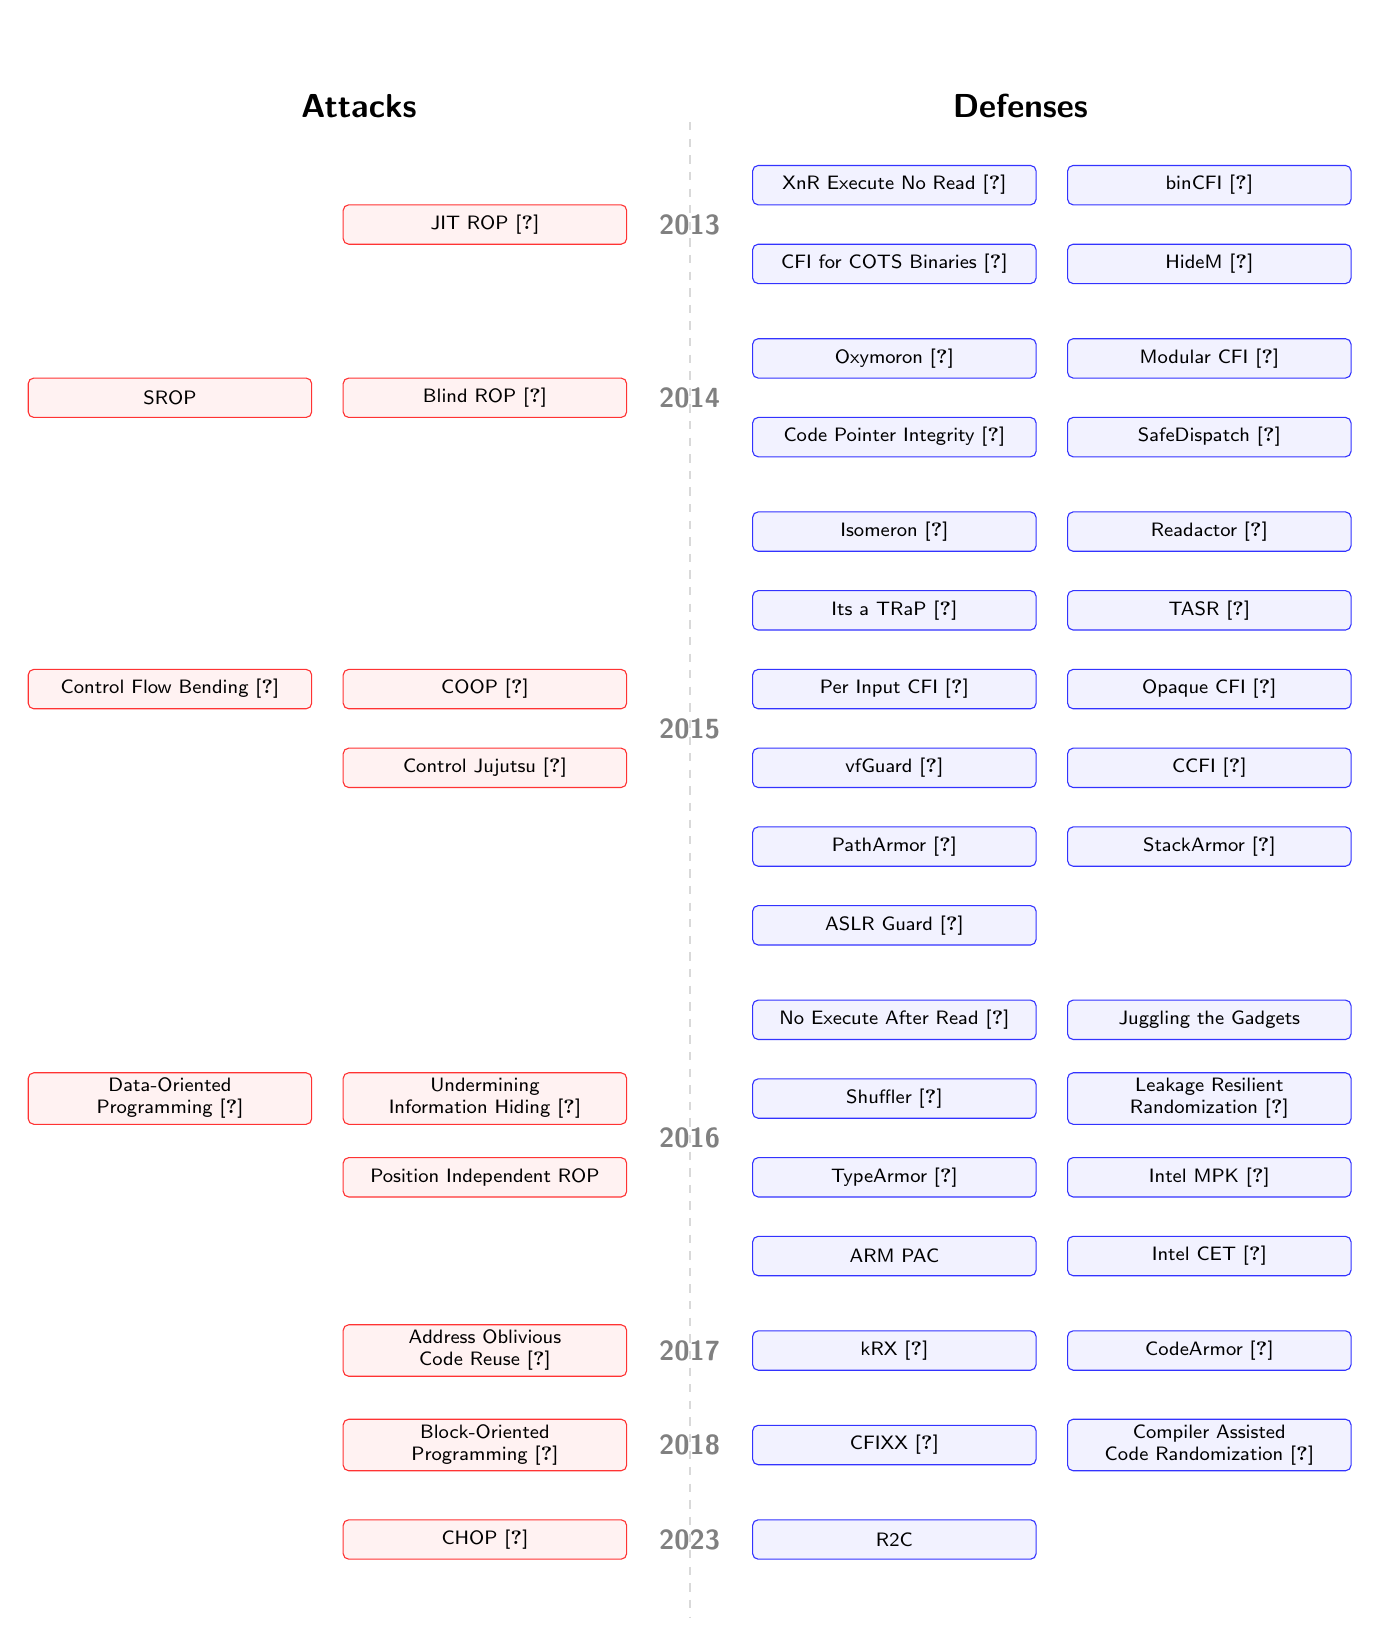
\begin{tikzpicture}[year node/.style={font=\bfseries\sffamily\color{gray}, align=center, inner sep=2pt},attack node/.style={draw=red!80, fill=red!5, rounded corners=2pt, font=\scriptsize\sffamily, align=center, minimum width=3.60cm, minimum height=0.5cm, inner sep=2pt, text width=3.40cm, execute at begin node=\setlength{\emergencystretch}{0pt}\tolerance 200\hyphenpenalty 10000\exhyphenpenalty 10000},defense node/.style={draw=blue!80, fill=blue!5, rounded corners=2pt, font=\scriptsize\sffamily, align=center, minimum width=3.60cm, minimum height=0.5cm, inner sep=2pt, text width=3.40cm, execute at begin node=\setlength{\emergencystretch}{0pt}\tolerance 200\hyphenpenalty 10000\exhyphenpenalty 10000},spine/.style={thick, gray!30, dashed}]%
\node[font=\large\bfseries\sffamily] at (-4.2,1.0) {Attacks};%
\node[font=\large\bfseries\sffamily] at (4.2,1.0) {Defenses};%
  % Year 2013%
\node[year node] at (0.0,-0.5) {2013};%
\node[attack node] at (-2.6,-0.5) {JIT ROP \allowbreak\cite{Snow2013}};%
\node[defense node] at (2.6,0.0) {XnR Execute No Read \allowbreak\cite{Backes2013}};%
\node[defense node] at (6.6,0.0) {binCFI \allowbreak\cite{zhang2013}};%
\node[defense node] at (2.6,-1.0) {CFI for COTS Binaries \allowbreak\cite{zhang2013}};%
\node[defense node] at (6.6,-1.0) {HideM \allowbreak\cite{Goktas2016b}};%
  % Year 2014%
\node[year node] at (0.0,-2.7) {2014};%
\node[attack node] at (-2.6,-2.7) {Blind ROP \allowbreak\cite{Bittau2014a}};%
\node[attack node] at (-6.6,-2.7) {SROP};%
\node[defense node] at (2.6,-2.2) {Oxymoron \allowbreak\cite{Backes2014f}};%
\node[defense node] at (6.6,-2.2) {Modular CFI \allowbreak\cite{niu2014a}};%
\node[defense node] at (2.6,-3.2) {Code Pointer Integrity \allowbreak\cite{Kuznetsov2014}};%
\node[defense node] at (6.6,-3.2) {SafeDispatch \allowbreak\cite{jang2014}};%
  % Year 2015%
\node[year node] at (0.0,-6.9) {2015};%
\node[attack node] at (-2.6,-6.4) {COOP \allowbreak\cite{Schuster2015a}};%
\node[attack node] at (-6.6,-6.4) {Control Flow Bending \allowbreak\cite{Carlini2015a}};%
\node[attack node] at (-2.6,-7.4) {Control Jujutsu \allowbreak\cite{Evans2015a}};%
\node[defense node] at (2.6,-4.4) {Isomeron \allowbreak\cite{Davi2015}};%
\node[defense node] at (6.6,-4.4) {Readactor \allowbreak\cite{Crane2015}};%
\node[defense node] at (2.6,-5.4) {Its a TRaP \allowbreak\cite{Crane2015b}};%
\node[defense node] at (6.6,-5.4) {TASR \allowbreak\cite{bigelow2015}};%
\node[defense node] at (2.6,-6.4) {Per Input CFI \allowbreak\cite{Niu2015}};%
\node[defense node] at (6.6,-6.4) {Opaque CFI \allowbreak\cite{Mohan2015}};%
\node[defense node] at (2.6,-7.4) {vfGuard \allowbreak\cite{Prakash2015}};%
\node[defense node] at (6.6,-7.4) {CCFI \allowbreak\cite{Mashtizadeh2015}};%
\node[defense node] at (2.6,-8.4) {PathArmor \allowbreak\cite{Goktas2016b}};%
\node[defense node] at (6.6,-8.4) {StackArmor \allowbreak\cite{Chen2015c}};%
\node[defense node] at (2.6,-9.4) {ASLR Guard \allowbreak\cite{Lu2015}};%
  % Year 2016%
\node[year node] at (0.0,-12.1) {2016};%
\node[attack node] at (-2.6,-11.6) {Undermining\\ Information Hiding \allowbreak\cite{Goktas2016}};%
\node[attack node] at (-6.6,-11.6) {Data{-}Oriented\\ Programming \allowbreak\cite{Hu2016}};%
\node[attack node] at (-2.6,-12.6) {Position Independent ROP};%
\node[defense node] at (2.6,-10.6) {No Execute After Read \allowbreak\cite{Werner2016}};%
\node[defense node] at (6.6,-10.6) {Juggling the Gadgets};%
\node[defense node] at (2.6,-11.6) {Shuffler \allowbreak\cite{WilliamsKing2016}};%
\node[defense node] at (6.6,-11.6) {Leakage Resilient\\ Randomization \allowbreak\cite{Braden2016}};%
\node[defense node] at (2.6,-12.6) {TypeArmor \allowbreak\cite{VanderVeen2015b}};%
\node[defense node] at (6.6,-12.6) {Intel MPK \allowbreak\cite{Wahbe1993}};%
\node[defense node] at (2.6,-13.6) {ARM PAC};%
\node[defense node] at (6.6,-13.6) {Intel CET \allowbreak\cite{IntelCET}};%
  % Year 2017%
\node[year node] at (0.0,-14.8) {2017};%
\node[attack node] at (-2.6,-14.8) {Address Oblivious\\ Code Reuse \allowbreak\cite{Rudd2017}};%
\node[defense node] at (2.6,-14.8) {kRX \allowbreak\cite{Pomonis2019}};%
\node[defense node] at (6.6,-14.8) {CodeArmor \allowbreak\cite{Chen2017a}};%
  % Year 2018%
\node[year node] at (0.0,-16.0) {2018};%
\node[attack node] at (-2.6,-16.0) {Block{-}Oriented\\ Programming \allowbreak\cite{Ispoglou2018}};%
\node[defense node] at (2.6,-16.0) {CFIXX \allowbreak\cite{Burow2018CFIXX}};%
\node[defense node] at (6.6,-16.0) {Compiler Assisted\\ Code Randomization \allowbreak\cite{Koo2018}};%
  % Year 2023%
\node[year node] at (0.0,-17.2) {2023};%
\node[attack node] at (-2.6,-17.2) {CHOP \allowbreak\cite{duta2023}};%
\node[defense node] at (2.6,-17.2) {R2C};%
\path[spine,draw] (0.0,0.8) -- (0.0,-18.2);%
\path[use as bounding box] (-8.40,-18.20) rectangle (8.40,2.00);%
\end{tikzpicture}
}%
    }
    \caption{Epoch timeline for dynamic attacks, semantic bypasses, and corresponding defenses (2013--present).}
    \label{fig:coevolution-epoch-dynamic-semantic}
\end{figure}
\section{Dynamic Attacks and Semantic Bypasses (2013--Present)}
\label{sec:epoch-dynamic-semantic}
The third epoch (2013--present) was driven by the realization that \emph{static} defenses cannot withstand \emph{dynamic} attacks.

In \citeyear{Snow2013} an attack called \gls{JITROP} showed that invalidating static a priori knowledge alone is insufficient.
\gls{JITROP} learns gadget locations by analyzing readable pointers into the code section.
In a second step, \gls{JITROP} uses this target-specific information to build a \gls{ROP} attack just in time, tailored to the target process memory layout.
A similar attack, called \gls{BROP}, exploits the behavior of certain server software to automatically respawn upon a crash~\cite{Bittau2014a}.
\gls{BROP} probes for valid gadget addresses by trying different addresses with brute force.

An attack called \gls{PIROP} showed that randomization that is too coarse-grained leaves randomized programs susceptible to partial address corruptions.
\gls{PIROP} exploits the fact that the relative distances between code units (\eg gadgets) below the randomization granularity remain constant.

As a response to \gls{JITROP} and \gls{BROP}, researchers upgraded their defenses to provide \emph{leakage-resilience}.
A key component in these defenses is to protect the randomized code with execute-only memory, thereby preventing an attacker from leaking a process' code section.
Early systems like \propername{XnR}~\cite{Backes2013} and \propername{HideM}~\cite{Giontaa2015} pioneered this approach by emulating execute-only pages in software or using split-TLB architectures.
\propername{Oxymoron} combined fine-grained randomization with execute-only memory while preserving code sharing between processes~\cite{Backes2014f}, and systems like \propername{\krx} extended these protections to the kernel~\cite{Pomonis2019}.
Execute-only memory comes in different variants, based on hardware support~\cite{Crane2015,luo2025}, with destructive code reads~\cite{Tang2015,Werner2016} or with compartmentalization~\cite{Braden2016}.
\propername{Readactor} combines fine-grained randomization with execute-only memory and \emph{booby traps}~\cite{Crane2015}.
Booby traps penalize an attacker for failed attack attempts by giving a clear signal of an ongoing attack~\cite{Crane2013,Crane2015b}.
Such a signal allows the attacked program to take counter-measures, such as preventing restarts or even retaliative action.
Taking a different approach, \propername{Isomeron} randomized the execution path rather than just the code layout by switching between diversified program variants at runtime~\cite{Davi2015}.

An alternative response to \gls{JITROP} is \emph{continuous re-randomization}.
\propername{Shuffler}, for example, re-randomizes the code layout at short intervals (50\,ms), introducing a tight deadline for disclosure~\cite{WilliamsKing2016}.
Similarly, \propername{TASR} rerandomizes at regular intervals, but instead of using a translation table, updates pointers in place~\cite{bigelow2015}.

Unable to disclose the code layout directly, a more sophisticated version of \gls{JITROP}---\emph{indirect} \gls{JITROP}---demonstrated the feasibility of inferring gadget locations from code pointers found on the stack~\cite{Davi2015,Crane2015}, which is commonly referred to as \emph{indirect information disclosure}.
In response to indirect information disclosure, \citeauthor{Crane2015} proposed \gls{CPH}~\cite{Crane2015}.
\gls{CPH} prevents disclosure by redirecting code pointers through a randomized trampoline table, located in execute-only memory.
However, \glsfirst{AOCR} demonstrated that attacks are still possible, even in the presence of \gls{CPH} or similar protection schemes~\cite{Rudd2017}.
Even without concrete information about gadgets, \gls{CPH} function pointers can be called using \emph{whole-function reuse}.
Thus, \gls{AOCR} directly challenges the \enquote{leakage resilience} postulated by Readactor.
Since the \gls{AOCR} attack is the main motivation for the defense presented in \cref{ch:r2c}, we will discuss its assumptions and principles in more detail in \cref{r2c:s:aocr}.

Just as static randomization failed against dynamic inspection, early implementations of \gls{CFI} were challenged by the inherent imprecision of static analysis and heuristics.
Because determining a precise \gls{CFG} is often undecidable, most \gls{CFI} solutions rely on an overapproximation of valid targets to avoid false positives.
This overapproximation gives attackers sufficient maneuverability to construct malicious execution paths that adhere to the previously determined allowed edges, as demonstrated by a series of attacks on \gls{CFI}~\cite{carlini2014,Carlini2015,Evans2015a,conti2015,Goktas2016b}.
An evaluation of \gls{CFI} implementations from \citeyear{li2020} shows that these issues are not merely theoretical and that some \gls{CFI} implementations even \emph{expand} the attack surface~\cite{li2020}.
Similarly, \citetitle{biondo2018} shows that implementation tradeoffs for performance can have unexpected consequences~\cite{biondo2018}.
Another related issue are semantic bypasses that target areas not covered by a \gls{CFI} solution.
For example, early \gls{CFI} defenses failed to take into account the semantics of dynamic dispatch in languages like \cpp, enabling attacks such as \gls{COOP}~\cite{Schuster2015a}.
\gls{COOP} uses virtual function calls to perform malicious computations, but from the perspective of a \cpp-oblivious \gls{CFI} \gls{COOP} stays within the legitimate \gls{CFG}.
\begin{listing}[t]
\begin{minted}{C++}
// The "Main Loop" Gadget (in existing code)
void dispatch(std::vector<Object*> &objs) {
    for (Object* obj : objs) {
        // Attacker controls 'obj' -> vtable
        obj->virtualFunc(); 
    }
}
\end{minted}
\caption{Example of a \gls{COOP} \enquote{Main Loop} gadget. An attacker can chain virtual calls by injecting a list of counterfeit objects.}
\label{lst:coop-gadget}
\end{listing}
In response, researchers have proposed \gls{CFI} solutions specialized for object-oriented languages~\cite{Gawlik2014,Zhang2015,Prakash2015,wang2018a,jang2014}.
\propername{CFIXX}, for instance, enforces strict object-type integrity on virtual calls to prevent COOP-style attacks~\cite{Burow2018CFIXX}.
Another semantic bypass called \gls{CHOP} focuses on stack unwinding and exception handlers~\cite{duta2023}.

To mitigate the shortcomings of static analysis, researchers have proposed further refinements of \gls{CFI}.
For example, \propername{OCFI} combines \gls{CFI} with code-layout randomization~\cite{Mohan2015}.
\propername{OCFI} uses the (now deprecated) MPX CPU extension to efficiently check targets against address ranges.
\propername{TypeArmor} addresses the problem of reconstructing the \gls{CFG} for binaries by considering function signatures as well~\cite{VanderVeen2015b}.
By instrumenting the program with dynamic binary instrumentation, \propername{TypeArmor} enforces conservatively determined lower and upper bounds on the number of function arguments.
\textpi{}CFI extends the traditional \enquote{code only} view of \gls{CFI} by taking concrete inputs into account~\cite{Niu2015}.
\propername{PathArmor} extends \gls{CFI} with context sensitivity by validating not only single call targets, but sequences of calls with the Intel \propername{Last Branch Register}.
\propername{OS-CFI} restricts valid call targets by taking the pointer origin into account, \eg the address-taken location of C function pointers~\cite{khandaker2019}.
\propername{CFI-LB} augments the statically determined \gls{CFG} with runtime context at the call site, such as a chain of return addresses on the stack~\cite{khandaker2019a}.
The technique behind \propername{CFI-LB} bears similarities with a concept related to fuzzer code coverage, which we will discuss in a later chapter (see \cref{psp:sec:motivation}).
Another challenge in \gls{CFG} construction is that it requires a holistic view of the entire program.
Modular control-flow integrity addresses this limitation by enabling the linkage of independently instrumented program modules~\cite{niu2014}.
Unfortunately, even precise \gls{CFG} construction cannot prevent attacks that stay entirely on legitimate control-flow paths.
\glsfirst{BOP} demonstrated that sufficiently large programs contain enough valid execution paths to construct malicious Turing-complete logic using only whole basic blocks~\cite{Ispoglou2018}.

Function returns (backward-edge control-flow transfers) are also challenging to restrict with static analysis, which is why most \gls{CFI} defenses use a different technique for returns.
The most robust form of backward-edge \gls{CFI} are shadow stacks~\cite{Burow2018a}.
A shadow stack is a separate stack in memory that holds copies of the return addresses on the regular stack.
Upon return, \gls{CFI} compares the return address on the regular stack with the return address on the shadow stack.
The motivation behind this separation is to isolate sensitive control-flow information (return addresses) from other data such as buffers.
Similar to the forward-edge case, shadow stacks must take into account semantic subtleties such as non-linear control-flow caused by C-style \code{setjmp} or \cpp exceptions.
When a \cpp function, for example, throws an exception, \cpp's stack-unwinding machinery unwinds the stack to the stack frame of a catching function (if any).

Researchers also attempted to generalize the separation of control-flow data by separating \enquote{safe} from \enquote{unsafe} data.
Techniques like \propername{StackArmor}~\cite{Chen2015c} and \gls{CPI}~\cite{Kuznetsov2014} follow this approach.
\gls{CPI}, for example, separates sensitive data like control-flow data and pointers from \eg potentially overflowing buffers.
\propername{Dataguard} later refined the policies deciding which stack objects should be separated~\cite{huang2022a}.
However, the security of this separation approach critically hinges on the protection of the isolated data against corruption and disclosure.
An initial attempt at protecting such a sensitive area in a performance-friendly way was hiding it in the vast address space of 64-bit systems.
This technique of hiding a safe area by randomizing its base address is known as \emph{information hiding}.
\propername{ASLRGuard}, for example, relies on information hiding to protect its \propername{AG-Stack}, a shadow stack implementation that includes indirect information disclosure in its threat model~\cite{Lu2015}.
Several attacks illustrate the limitations of information hiding~\cite{Goktas2016,Evans2015,Oikonomopoulos2016a}.
Even without pointer leaks, information hiding is susceptible to leakage.
By using memory allocation side-channels, attackers can disclose the safe area location.
A technique called stack spraying, for example, successfully reveals the hidden stack of code-pointer integrity~\cite{Kuznetsov2014}.
\propername{SafeHidden} attempted to harden information hiding against probing attacks by dynamically re-randomizing the safe area upon detecting suspicious memory access patterns~\cite{wang2019a}.
A more robust way to protect the sensitive area for shadow stacks is to rely on hardware features such as Intel CET or Intel MPK.
CET implements shadow stacks in hardware, whereas MPK allows the protection of arbitrary memory regions with secret keys.

\gls{CCFI} chose a different approach to enforce the \gls{CFI} policy~\cite{Mashtizadeh2015}.
Instead of instrumenting the program to check control-flow transfers against a statically computed \gls{CFG}, \gls{CCFI} cryptographically encrypts control-flow data with a \gls{HMAC}.
\gls{CCFI} provides strong security guarantees, but \gls{CCFI} incurs a significant performance overhead (up to 2.5x) and requires 12 vector registers for the cryptographic key.
The \gls{CCFI} approach was later implemented in hardware in the form of ARM's \gls{PAC}.
While \gls{CCFI} chose to outline \gls{HMAC}s into a separate table to deal with values greater than 64 bits, \gls{PAC} reuses up to 31 bits of a pointer's address upper bits to store the \gls{HMAC}.
This inlining also means, however, that the security provided by \gls{PAC} is limited by the available bits in a memory address.
This limitation makes \gls{PAC} vulnerable to cryptographic attacks, in particular offline attacks~\cite{li2022}.


To address the prohibitive overhead of full memory safety, researchers explored ways to trade precision for performance.
Techniques like \propername{Low-Fat Pointers}~\cite{kwon2013} and \propername{Delta Pointers}~\cite{kroes2017,Kroes2018} optimized metadata checks to reduce the cost of spatial safety.
Other approaches abandoned spatial enforcement entirely to focus solely on temporal safety, which can often be enforced more efficiently~\cite{dang2017a,vanderkouwe2017,lee2015}.
Despite these optimizations, software-based memory safety typically still incurs overheads that hinder widespread adoption in production systems.

\section{Transient Execution Attacks (2018--Present)}
\label{sec:epoch-transient}
In 2018, the disclosure of \propername{Spectre} and \propername{Meltdown} marked a paradigm shift in system security.
These \emph{transient execution attacks} exploit microarchitectural side-channels to leak data across protection boundaries, fundamentally challenging the assumption that architectural isolation implies security.
This discovery drew significant attention away from classical \glspl{CRA}, with researchers trying to understand and mitigate this new class of threats.
While \glspl{TEA} represent a critical threat to data confidentiality, they are not \glspl{CRA} in the traditional sense; they do not typically aim to hijack control flow to execute arbitrary code, but rather to leak information.
However, as demonstrated by \gls{JITROP} and \gls{AOCR}, information leakage is often the precursor to a successful control-flow hijack.
Despite the shift in focus towards microarchitectural defenses, the architectural vulnerabilities allowing for \gls{ROP}, \gls{COP}, and data-oriented attacks remain a critical threat.
As the \gls{AOCR} attack demonstrates, even with modern mitigations, the coupling of code and data remains a critical weakness that attackers can exploit without needing to trigger transient execution.

\section{Summary}

This chapter has traced decades of co-evolution between code-reuse attacks and defenses.
Each epoch reveals a recurring pattern: a new defense closes one attack vector, only to be circumvented by attackers exploiting a different assumption.
Code injection was stopped by \gls{DEP}, \gls{ROP} prompted both \gls{CFI} research and fine-grained randomization, and advanced attacks like \gls{COOP} and \gls{JITROP} exposed gaps in existing \gls{CFI} and randomization techniques.

While the defense categories examined in this chapter target various stages of the attack lifecycle, a holistic solution remains elusive.
Memory-safety enforcement thwarts corruption at the point of origin, yet the performance costs of achieving exhaustive spatial and temporal safety are often prohibitive.
\gls{CFI} acknowledges the likely presence of corruption but is constrained by the inherent imprecision of static analysis and gaps in semantic coverage.
Leakage-resilient randomization, while complicating attacker reconnaissance, still fails to eliminate all inference-based exploitation vectors.
In the following chapter we address a critical weakness in randomization-based defenses: the predictability of observable data that enables inference-based exploitation.
